\chapter{Methods for solving QUBO problems}

\label{review}
\vspace{2em}
There are a variety of possible methods for solving QUBO problems and Ising models which can be broadly categorized as Classical, Quantum Annealing, Neural Network Quantum States, and Hybrid Quantum-Classical Algorithms.

\section{Classical}
Classical approaches search for solutions without exploiting quantum properties such as the superposition of states. A typical classical approach to solving large QUBO problems is by exact diagonalization of the corresponding Ising Hamiltonian~\cite{b25}. Exact diagonalization solves for all the eigenvalues and eigenvectors by diagonalizing the corresponding Ising Hamiltonian matrix. This is also known as the eigendecomposition of a matrix and is possible for all Hermitian matrices, which are those that represent the Hamiltonian of a quantum system~\cite{b27}. However, the runtime of exact diagonalization scales exponentially with input problem size and becomes computationally infeasible once the matrix grows large \cite{b25}. Since we are only interested in finding the smallest eigenvalue and the corresponding eigenvector, we can use iterative methods such as the Lanczos algorithm or the implicitly restarted Arnoldi method to find the smallest eigenvalue~\cite{b28,b29}. However, such methods also often run into stability issues. The rapidly increasing search space for QUBO problems has inspired classical methods that aim to efficiently find approximate solutions to QUBO problems instead.

One class of such methods relies on "heuristics" to search for optimal solutions~\cite{b12}. For example, variants of Tabu search---a local search algorithm that allows for moves that are not improvements and discourages visiting already visited states---are highly competitive heuristic algorithms to find good solutions to QUBO problems\cite{b2,b30}. Dunning et al.\yrcite{b12} conducted a systematic review and evaluation of published heuristics for QUBO problems and provided an open-source problem repository MQLib for further research. 
%In addition, the solver by Dunning et al.\cite{b12} also provides a machine-learning model that predicts the best-performing set of heuristics for a given problem input.

Another classical approximate method for solving QUBO problems is simulated annealing (SA) \cite{KATAYAMA2001103}. Simulated annealing \cite{Kirkpatrick} is a probabilistic method for approximating the global minimum of a function. The main idea of SA is to start with an initial trial state and a temperature $T$ which decreases slowly during the search. In each iteration, the algorithm samples neighboring solutions of the current state and probabilistically accepts the new state based on the difference in energy, $\Delta E$, between the current state and the new state. If $\Delta E < 0$, then the new state is always accepted and if $\Delta E \geq 0$, the new solution is accepted with probability $\propto e^{-\frac{\Delta E}{T}}$. The algorithm to sample new states is adapted from the Metropolis-Hastings sampling method \cite{metropolissampling} and the chance to explore poorer solutions allows for the algorithm to escape local minima.

There are many more classical approaches to solving QUBO problems as it has been studied extensively. For a detailed survey of classical methods for solving QUBO problems, refer to \cite{punnen2022quadratic}.

\section{Quantum Annealing}\label{section:annealing}
Quantum annealing, first formulated by Kadowaki and Nishimori \yrcite{kadowaki1998quantum}, can solve for the ground state configuration of Ising models by utilizing the \textit{adiabatic theorem}. The \textit{adiabatic theorem} states that "a quantum system in its ground state will remain in the ground state, provided that the Hamiltonian governing the dynamics changes sufficiently slowly" \cite{b14,b15}. If we can manipulate the final Hamiltonian of a quantum system to one that describes the Ising model of interest, we can find the ground state of the Ising model simply by measuring the final configuration of the quantum system.

\begin{figure}[h!]
    \centering
    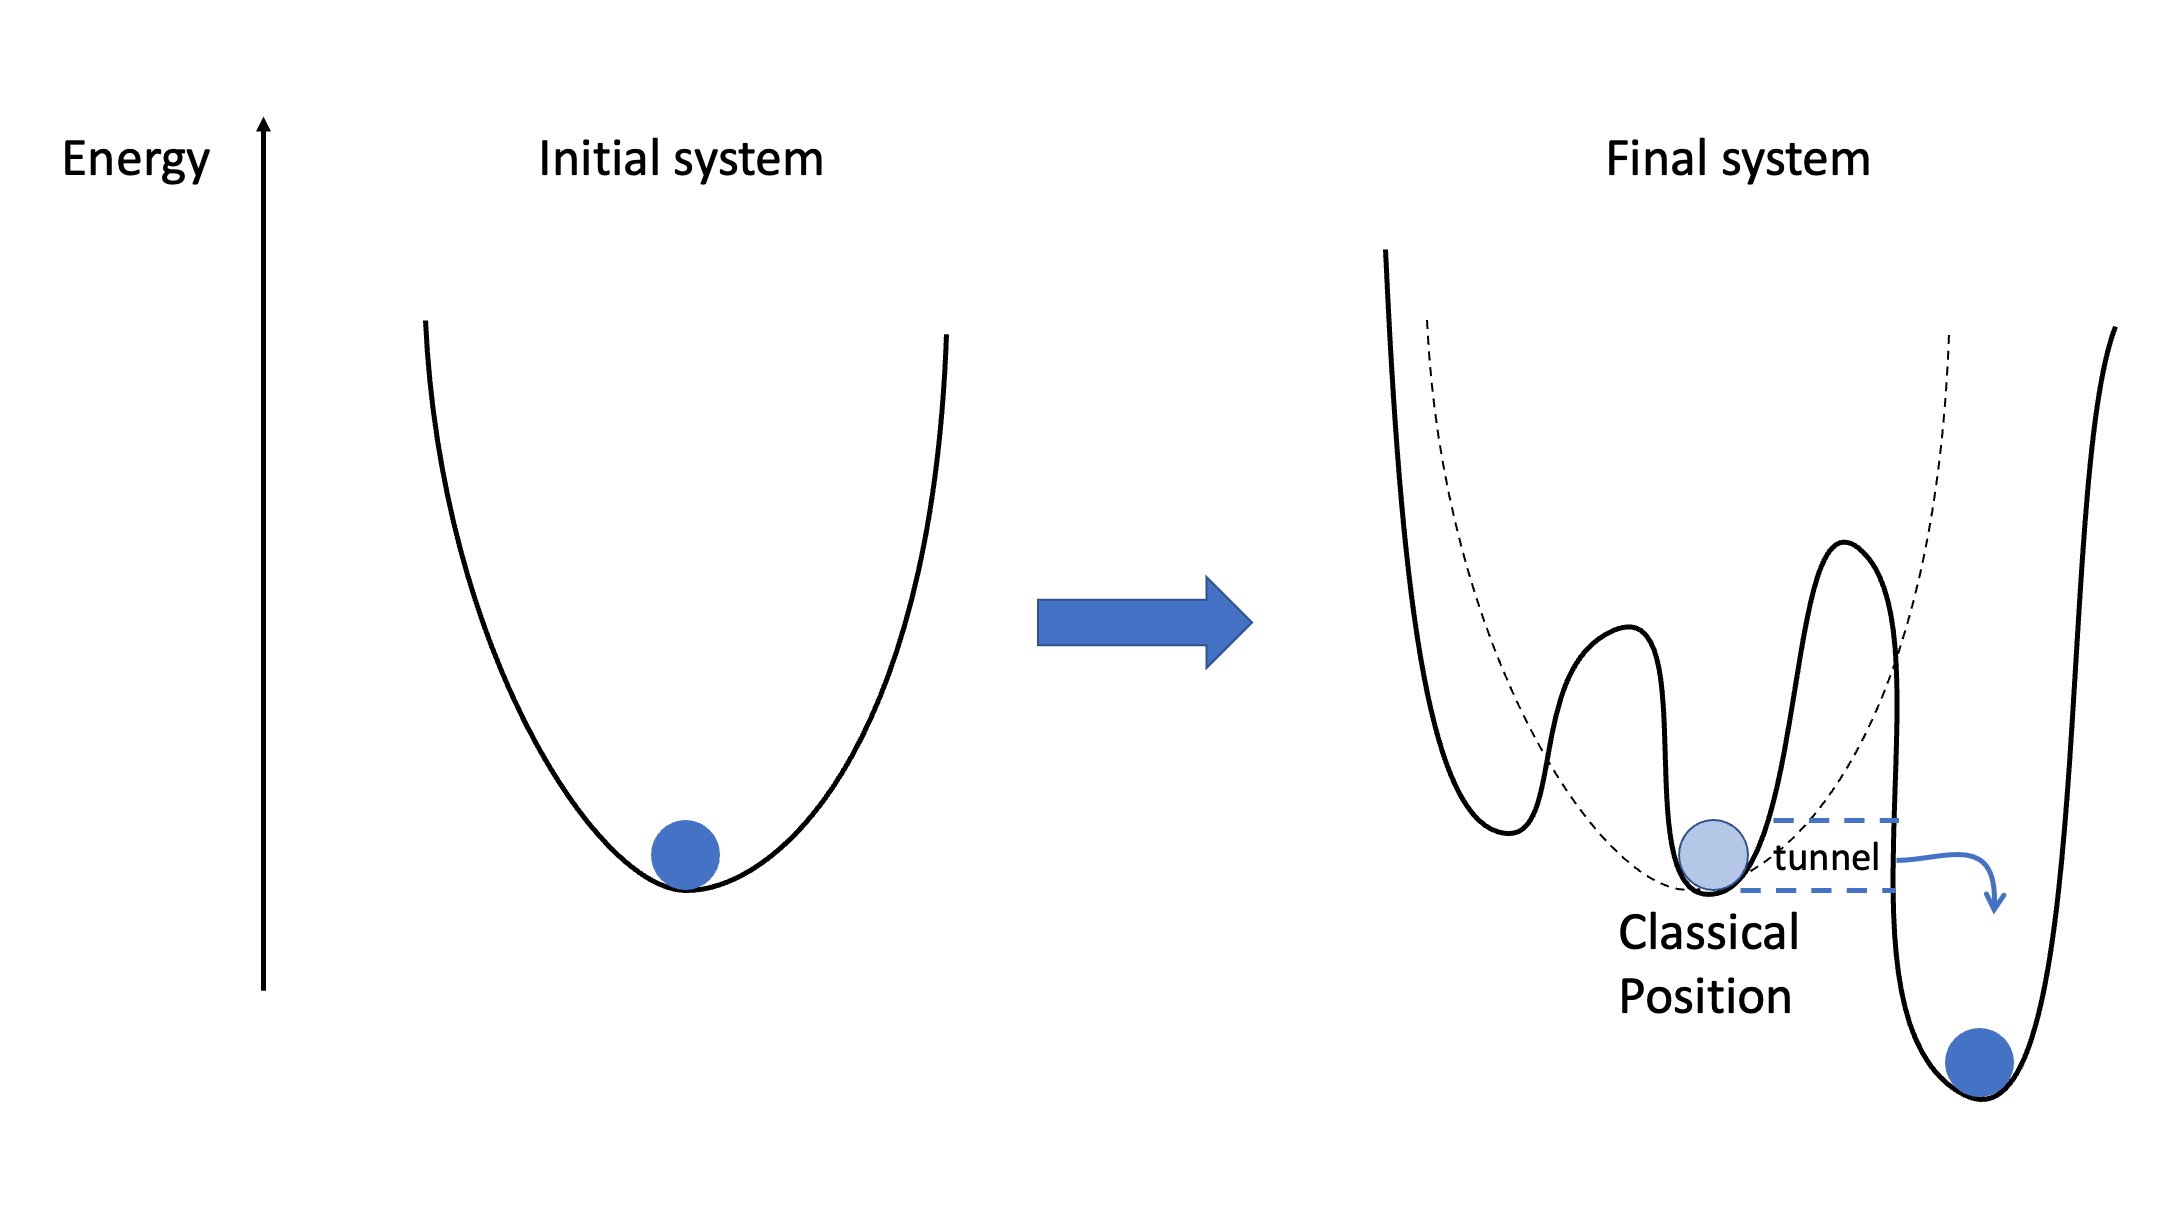
\includegraphics[width=0.8\linewidth]{images/quantum_annealing.png}
    \caption{Energy landscape before (left) and after (right) quantum annealing}
    \label{quantumannealing}
\end{figure}

Quantum annealers first prepare a system in the ground state with a simple initial Hamiltonian $H_0$ (called the mixer or tunneling Hamiltonian), shown with a simple energy landscape in the left of \autoref{quantumannealing}. Then, the system Hamiltonian is slowly changed to a more complex form $H_c$ \cite{b10}, shown with a complex energy landscape in the right of \autoref{quantumannealing}. The Hamiltonian at any point $H(s)$ can be written as
\begin{equation}
    \label{eqn:annealinghamiltonian}
    H(s) = A(s)H_0 + B(s)H_c
\end{equation}
where $s \in [0,1]$ is the normalized anneal fraction and $A(s)$ and $B(S)$ are decreasing and increasing functions respectively and are determined by the specific quantum annealing controls. At the start of the annealing we should have $A(s) >> B(s)$ and at the end of the annealing we should have $B(s) >> A(s)$. If the transition time is sufficiently large, the adiabatic theorem ensures that the system will remain in the ground state which can then be measured to yield the desired ground state configuration of $H_c$ \cite{b14}. 

As $H_0$ usually consists of a transverse magnetic field and does not commute with the target Hamiltonian $H_c$, it allows for quantum tunneling through energy barriers between classical states \cite{kadowaki1998quantum}. This allows for the wave function to remain at the ground state even when classical search methods may end up stuck in a local minimum. However, the adiabatic theorem requires an arbitrarily long anneal time to guarantee that the system remains in the ground state which is not feasible for practical purposes. Current implementations of quantum annealing instead rely on a finite time approximation with repeated sampling to increase the success rate \cite{farhi2001}.

Quantum annealing has been extensively studied and applied in multiple fields such as Scheduling Problems \cite{b17}, Portfolio Optimization \cite{b18} and Quantum simulations \cite{b19}. Even though there are significant roadblocks in scaling the currently limited hardware capabilities \cite{b14} and it is debated whether Quantum Annealing will run faster than classical search methods \cite{b10}, there is hope that these challenges can be tackled soon with the rapid progress made in quantum computing research. At present, the leading commercial provider of quantum annealing hardware is D-wave, a Canadian quantum computing company \cite{b16}.

\section{Neural-Network Quantum States}
Carleo and Troyer \cite{b20} introduced a neural-network-based method for modeling the wave function of a target quantum system known as \textit{neural-network quantum states} (NNQS). The authors used the approach to find the ground state and time evolution of the Ising and Heisenberg models in Physics. The NNQS is used as an Ansatz to approximate the wave function, which can be viewed as a complex probability distribution, of a system as an artificial neural network \cite{b25}. The more general method of using an Ansatz as a trial wave function and minimizing its energy through Monte Carlo sampling is also known as variational Monte Carlo (VMC).

The theoretical foundations of the ability of NNQS to approximate a wave function rely on the Kolmogorov–Arnold representation theorem \cite{kolmogorov1957representation}, which implies that every multivariate, smooth function can be represented by a neural network with two hidden layers. Since the wave function of a quantum system generally satisfies these requirements, we can expect that a neural network can reasonably approximate the wave function of the system \cite{b20}.

\begin{figure}[h!]
    \centering
    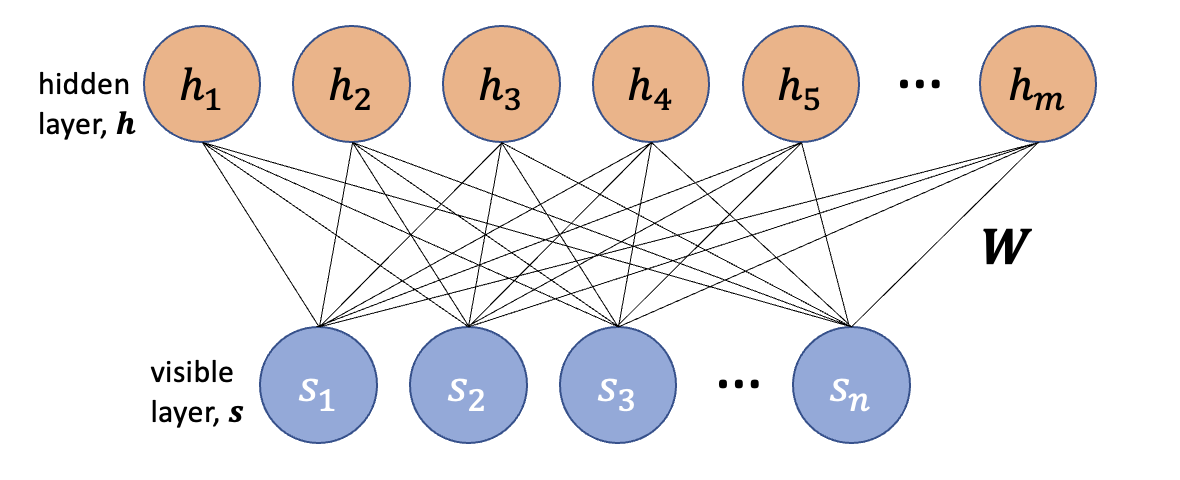
\includegraphics[width=0.9\linewidth]{images/rbm_diagram.png}
    \caption{Structure of Restricted Boltzmann Machine}
    \label{rbmstructure}
\end{figure}

The original NNQS architecture utilized a Restricted Boltzmann Machine (RBM) as its network \cite{b20}. The RBM, shown in \autoref{rbmstructure}, is an energy-based generative model that has two layers of nodes, a visible layer $\boldsymbol{s}$ with $n$ nodes, a hidden layer $\boldsymbol{h}$ with $m$ nodes, and a weight matrix $\mathbf{W}$. The number of hidden nodes is generally a multiple of the number of visible nodes and the ratio $\alpha = \frac{m}{n}$ is a hyperparameter of the model. Each visible node $s_i$ is connected to every hidden node $h_j$ with a certain weight $W_{ij}$ but there are no connections within the visible or hidden layer. In other words, the visible and hidden nodes of the RBM form a bipartite graph.

When approximating the wave function of an Ising model, each visible node $s_i$ is used to represent the spin of a particle in the Ising model and can only take on the values of $1$ and $-1$ \cite{b20}. The representation of the wave function by the RBM can be expressed as:
\begin{equation}
    \Psi(\boldsymbol{s} ; \boldsymbol{\theta}_{rbm}) = \sum_{h} e^{\sum_i a_s s_i + \sum_j b_j h_j + \sum_{i,j}W_i s_i h_j} 
\end{equation}
where  $\boldsymbol{\theta}_{rbm} = \{\boldsymbol{a}, \boldsymbol{b}, \boldsymbol{W}\}$ are the biases and weights of the RBM \cite{b20}. The RBM is trained in an unsupervised manner. The network weights $\mathbf{W}$ are usually updated by performing Gibbs sampling, calculating the average energy of sampled configurations, and using gradient-based optimization algorithms \cite{b25}.

\begin{figure}[h!]
    \centering
    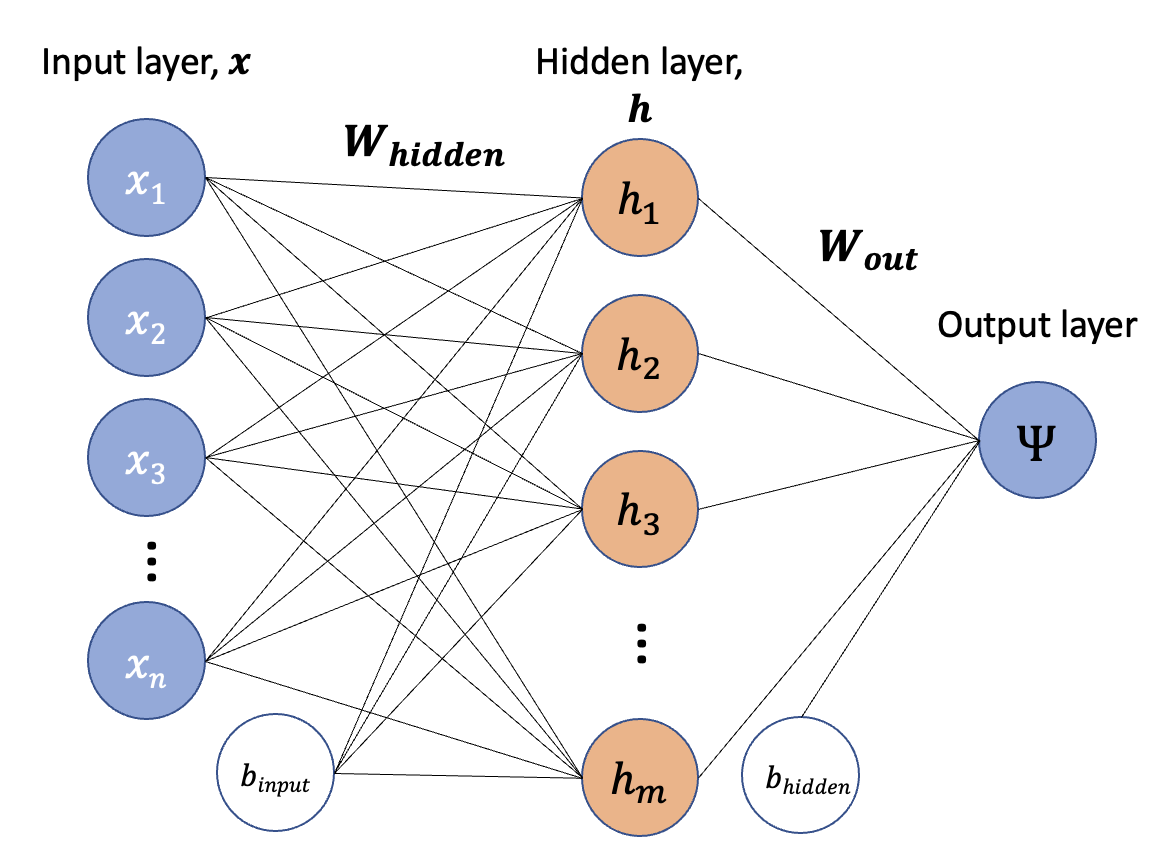
\includegraphics[width=0.7\linewidth]{images/mlp_diagram.png}
    \caption{Structure of Multilayer Perceptron with 1 hidden layer and 1 real-valued output node}
    \label{rbmstructure}
\end{figure}

Other neural network architectures such as the Multilayer Perceptron (MLP) can also be used in NNQS. An MLP model is a feedforward artificial neural network that consists of an input layer $\boldsymbol{x}$, one or more hidden layers, and an output layer. Each layer is fully connected to the next layer with certain weights and each node has a non-linear activation function $\sigma$ such as the sigmoid or ReLU function. Each input node $x_i$ represents the spin of a particle in the Ising model and the output nodes represent the value of the wave function. If we assume that the wave function is real and positive, then only one output node is needed to represent the real part of the wave function. \cite{b20}. With a complex wave function, we could employ output combinations with two nodes representing either the real and imaginary components or the magnitude and phase. With one hidden layer, the MLP representation of the wave function can be expressed as:
\begin{equation}
    \Psi(\boldsymbol{x}; \boldsymbol{\theta}_{mlp}) = 
    \sigma_{out} \left(
    \boldsymbol{W}_{out} \hspace{2px}
    \sigma_{hidden} \left( \boldsymbol{W}_{hidden}\boldsymbol{x} + \boldsymbol{b}_{input} \right) + \boldsymbol{b}_{hidden} \right)
\end{equation}
where  $\boldsymbol{\theta}_{mlp} = \{\boldsymbol{W}_{hidden}, \boldsymbol{b}_{input}, \boldsymbol{W}_{out}, \boldsymbol{b}_{hidden}\}$ are the weights and bias of the MLP and $\sigma_{out}, \sigma_{hidden}$ are the non-linear activation functions of the nodes \cite{b20}. The MLP is trained in an unsupervised manner, similar to the RBM, except that a more general sampling method, the Metropolis-Hasting algorithm, is used \cite{b25}.

\section{Hybrid quantum-classical}
The fourth class of QUBO solving methods are hybrid quantum-classical methods which are designed to make use of current limited quantum computing resources by integrating them with classic methods to solve combinatorial optimization problems \cite{b32}. In the noisy intermediate-scale quantum (NISQ) era that we are currently in, quantum computers are not yet stable enough to be able to reliably run deep and complex quantum circuits. 

\begin{figure}[h!]
    \centering
    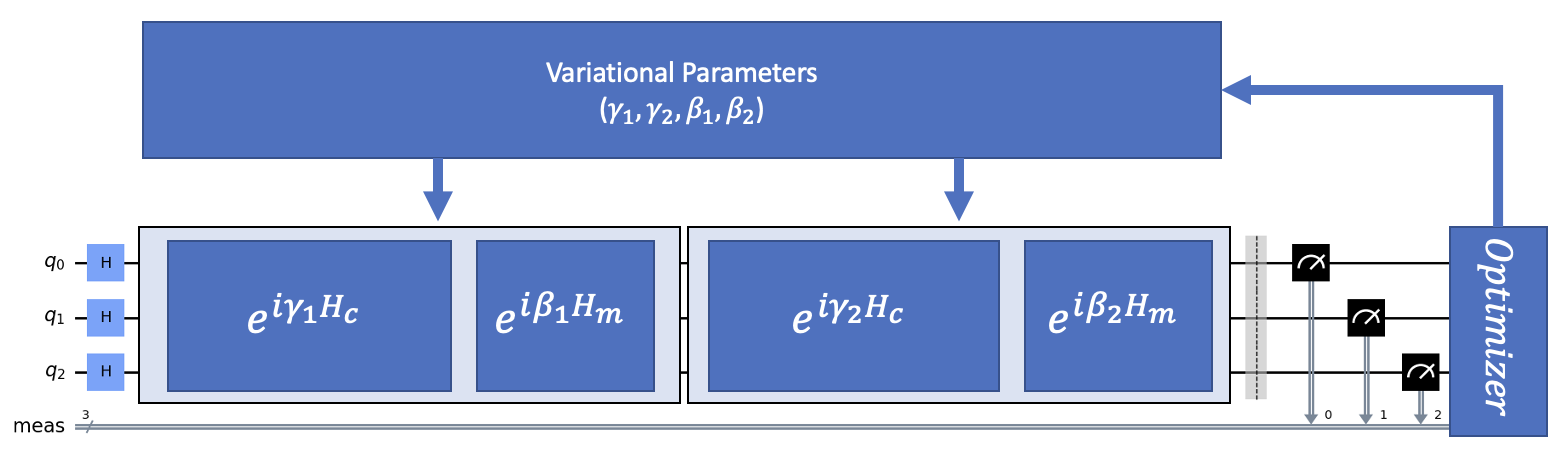
\includegraphics[width=\linewidth]{images/qaoa_circuit.png}
    \caption{Circuit diagram of the QAOA algorithm with $p=1$}
    \label{qaoacircuit}
\end{figure}

One such algorithm is the Quantum Approximate Optimization Algorithm (QAOA) which is used to find approximate solutions to general combinatorial optimization problems \cite{b23}. Similar to NNQS, QAOA aims to find an approximation of the ground state of an input Hamiltonian using gate-based quantum circuits and $2p$ parameters which are optimized with a classical computer \cite{b34}. With a problem of size $N$. the algorithm first prepares a quantum state $| + \rangle^{\otimes N}$ in uniform superposition by applying the Hadamard gate to each of the $n$ inputs \cite{b34}. The trial wave function is then constructed by
\begin{equation}
    \Psi(\boldsymbol{\gamma}, \boldsymbol{\beta}) = U_B(\beta_p) U_C(\gamma_p)...U_B(\beta_1) U_C(\gamma_1) | + \rangle^{\otimes N}
\end{equation}
\begin{align*}
    U_C(\gamma) &= e^{-i\gamma H_c} \\
    U_B(\beta) &= e^{-i\beta H_0}
\end{align*}
Using the time-independent Schrödinger equation, we can see that $U_c$ and $U_B$ are operators that evolve the state with the Hamiltonian $H_c$ (problem Hamiltonian) and $H_0$ (an easy-to-implement, mixing Hamiltonian) for time intervals $\boldsymbol{\gamma}$ and $\boldsymbol{\beta}$ while the parameter $p$ determines the number of independent parameters of the final state \cite{b34}. The state is then measured and $\boldsymbol{\gamma}$ and $\boldsymbol{\beta}$ are chosen to minimize the average energy of the sample measurements. With the optimal parameters, the final solution can then be determined by repeatedly sampling from the trial wave function.

There is evidence that QAOA is more difficult for classical computers to simulate compared to Quantum Annealing which may suggest that it could be a better way to demonstrate quantum supremacy \cite{farhi2016quantum}. In contrast to quantum annealing which can only be run on specialized quantum annealing devices, QAOA can be implemented on a general gate-based quantum computer \cite{b22}. 